\documentclass[c,8pt,xcolor...,x11names]{beamer}
\usepackage{icclslides}
\usepackage[latin1]{inputenc}
\usepackage[british]{babel}
\usepackage{amssymb}
\usepackage{latexsym}
\usepackage{rotate}
\usepackage{tikz}
\usepackage{verbatim}
\usepackage{colortbl}
\usepackage{booktabs}
\usepackage{ulem}
% \usepackage{arydshln}
\usepackage{pdfpages}
\usepackage{graphicx} 
\usepackage{tikz}
\usetikzlibrary{positioning}

\tikzstyle{ele} = [circle, text centered, minimum width=1em, minimum height=3ex]

%% Uncomment to activate navigation symbols in the lower right of the pages:
\setbeamertemplate{navigation symbols}{}

\renewcommand{\Myauthor}{Aldo [family name], Tobias John, Patrick Wienhöft}
\renewcommand{\Mytitle}{The boolean Pythagorean Triples problem}


\author{Aldo Kurmeta\\ Tobias John\\ Patrick Wienhöft}

\title{\Mytitle}

\subtitle{subtitle}

%\logo{\includegraphics{logo-tu-ilmenau.jpg}}

\institute{TU Dresden}

\date{date of the presentation}

\usepackage{showexpl} 

\lstloadlanguages{[LaTeX]Tex} 
\lstset{% 
	basicstyle=\ttfamily\small, 
	commentstyle=\itshape\ttfamily\small, 
	showspaces=false, 
	showstringspaces=false, 
	breaklines=true, 
	breakautoindent=true, 
	captionpos=t 
} 

\begin{document} 
	
% alternative title frame
%	\begin{frame}
%	\customtitle
%	\begin{list2}
%		\item What is {\sc Beamer}?
%		\item How to produce a presentation?
%		\item How to create overlays?
%	\end{list2}
%\end{frame}


% title frame
\maketitle


% Aldo's part
\section{Introduction}
\begin{frame}{Example}

	% this is just an idea for an example
	\begin{itemize}
		\item Set of Integers: $ \{1, \ldots, 15\}  $
		\pause
		\item Triples: 
		\begin{flalign*}
		3^2 + 4^2 &= 5^2 &\\ 
		6^2 + 8^2 &= 10^2 &\\
		9^2 + 12^2 &= 15^2 &\\
		5^2 + 12^2 &= 13^2
		\end{flalign*}
		\pause
		\item Partition: $ \{1,2,3,4,6,7,8,9,11,12,14 \}, \{5, 10, 13, 15\}  $
	\end{itemize}
	
	
	
\end{frame}

\section{Quick history of the problem}


% Patrick's part
\section{Framework}

%TODO tikz

\section{Encoding}

\begin{frame}{Encoding - Intuition}
	Idea:
	\begin{itemize}
		\item one variable for each number
		\pause
		\item one constraint clause for each Pythagorean triple
		\pause
		\item interpretation gives partition
	\end{itemize}
\end{frame}

\begin{frame}{Encoding}
	Binary Pythagorean triple problem with $n$ numbers \\
	\vspace{5px}
	\pause
	Set of variables $V = \{ p_k \quad | \quad 1 \leq k \leq n \}$ \\
	\vspace{5px}
	\pause
	Constraint for non-equality: $NotEqual(x,y,z) = (x \vee y \vee z) \wedge (\neg x \vee \neg y \vee \neg z) $ \\
	\vspace{5px}
	\pause
	Constraint for all Pythagorean triples: $F = \bigwedge\limits_{\small\substack{1 \leq x,y,z \leq n \\ x^2+y^2=z^2}} NotEqual(p_x,p_y,p_z)$ \\
	\vspace{10px}
	\pause
	For an interpretation $I \subseteq V$ with $I \models F$, the resulting partition is:
	\begin{itemize}
		\item $ P_1 = \{ x \quad | \quad p_x \in I \}$
		\item $ P_2 = \{ x \quad | \quad p_x \notin I \} $
	\end{itemize}
\end{frame}

\begin{frame}{Encoding - Example}
	As in beginning example, $n=15$ \\
	\vspace{5px}
	\pause
	$V = \{ p_1, p_2, \dots ,p_{15} \}$
	\pause
	\begin{flalign*}
		F \quad = & \quad \quad (p_3 \vee p_4 \vee p_5) \wedge (\neg p_3 \vee \neg p_4 \vee \neg p_5) &\\
		& \wedge \quad (p_6 \vee p_8 \vee p_{10}) \wedge (\neg p_6 \vee \neg p_8 \vee \neg p_{10}) &\\
		& \wedge \quad (p_9 \vee p_{12} \vee p_{15}) \wedge (\neg p_9 \vee \neg p_{12} \vee \neg p_{15}) &\\
		& \wedge \quad (p_5 \vee p_{12} \vee p_{13}) \wedge (\neg p_5 \vee \neg p_{12} \vee \neg p_{13}) &
	\end{flalign*}
	
	\pause
	Possible interpretation: $I = \{p_5, p_{10}, p_{13}, p_{15}\}$ \\
	\vspace{5px}
	\pause
	Resulting partition:
	\begin{itemize}
		\item $P_1 = \{1,2,3,4,6,7,8,9,11,12,14\}$
		\item $P_2 = \{5,10,13,15\}$
	\end{itemize}
\end{frame}

\section{Transformations}

\begin{frame}{Transformation}
	Goal: from $F$, find formula $F'$ which
	\begin{itemize}
		\item is easier to solve
		\pause
		\item preserves satisfiability
		\pause
		\item has models that can be easily transformed into models for $F$
	\end{itemize}
	\vspace{5px}
	\pause
	Approaches:
	\begin{itemize}
		\item eliminate clauses with variables only occuring once
		\pause
		\item break partition symmetry
	\end{itemize}
\end{frame}

\begin{frame}{Clause elimination}
	\begin{flalign*}
		F \quad = & \quad \quad NotEqual(p_3,p_4,p_5) &\\
		& \wedge \quad NotEqual(p_6,p_9,p_{12}) &\\
		& \wedge \quad NotEqual(p_9,p_{12},p_{15}) &\\
		& \wedge \quad NotEqual(p_5,p_{12},p_{13}) &
	\end{flalign*}
	Note $p_3$ only occurs in $NotEqual(p_3,p_4,p_5)$ and thus does not affect any other clauses
	\vspace{5px}
	\pause
	\begin{itemize}
		\item if $p_4^I \neq p_5^I$ then $NotEqual(p_3,p_4,p_5)$ is satisfied
		\pause
		\item if $p_4^I = p_5^I = \top$ then choose $p_3^I = \bot$
		\pause
		\item if $p_4^I = p_5^I = \bot$ then choose $p_3^I = \top$
	\end{itemize}
	\vspace{5px}
	\pause
	$\rightarrow$ clause $NotEqual(p_3,p_4,p_5)$ will not cause conflict
	\vspace{5px}
	\pause
	\begin{flalign*}
		F' \quad = & \quad \quad NotEqual(p_6,p_9,p_{12}) &\\
		& \wedge \quad NotEqual(p_9,p_{12},p_{15}) &\\
		& \wedge \quad NotEqual(p_5,p_{12},p_{13}) &
	\end{flalign*}
\end{frame}

\begin{frame}{Clause elimination}
	Notes:
	\begin{itemize}
		\item $F'$ might have more models than $F$
		\pause
		\item choice for variables occurring only once in $F$ is important but not represented in $F'$
		\pause
		\item $\rightarrow$ remember deleted clauses and modify interpretation of $F'$ accordingly
	\end{itemize}
	
	\vspace{5px}
	\pause
	Example:

	\begin{itemize}
		\item deleted clause $NotEqual(p_3,p_4,p_5)$ because $p_3$ only occurred once
		\pause
		\item $I' \models F'$ and $\{p_3,p_4,p_5\} \subseteq I'$
		\pause
		\item $I = I' \setminus {p_3}$
		\item while $I' \not\models F$, we have $I \models F$
	\end{itemize}
\end{frame}

\begin{frame}{Breaking Symmetry}
	\begin{itemize}
		\item formulas $F$ and $F'$ are symmetric
		\pause
		\item if $I \models F'$ then $V \setminus I \models F'$
		\pause
		\item $\rightarrow$ introduce unit clause for variable occurring in $F'$
		\item $F'' = F' \wedge p_x$
	\end{itemize}
	\vspace{5px}
	\pause
	Note that every model for $F''$ is a model for $F'$ and the transformation is satisfiability preserving
\end{frame}


% Tobias' part
\section{Cube-and-conquer solving}
\begin{frame}{Cube-and-conquer solving}
	\begin{itemize}
		\item Problem: solving with conflict-driven clause leraning (CDCL) is too slow
		\pause
		\item Solution: use different heuristics $\Rightarrow$ cube-and-conquer solver (C\&C)
	\end{itemize}
	\pause
	\begin{figure}
		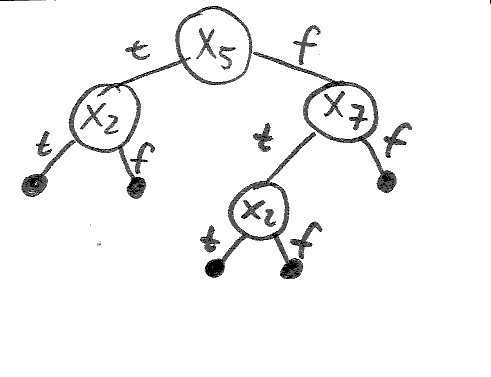
\includegraphics[width=0.5\textwidth]{images/scan1.png} 
		%\caption{Binary branching tree}
	\end{figure}
\end{frame}

\begin{frame}{Runtime}
	\begin{itemize}
		%TODO: add runtime of the algorithm
		\item x time
	\end{itemize}
	\begin{figure}
		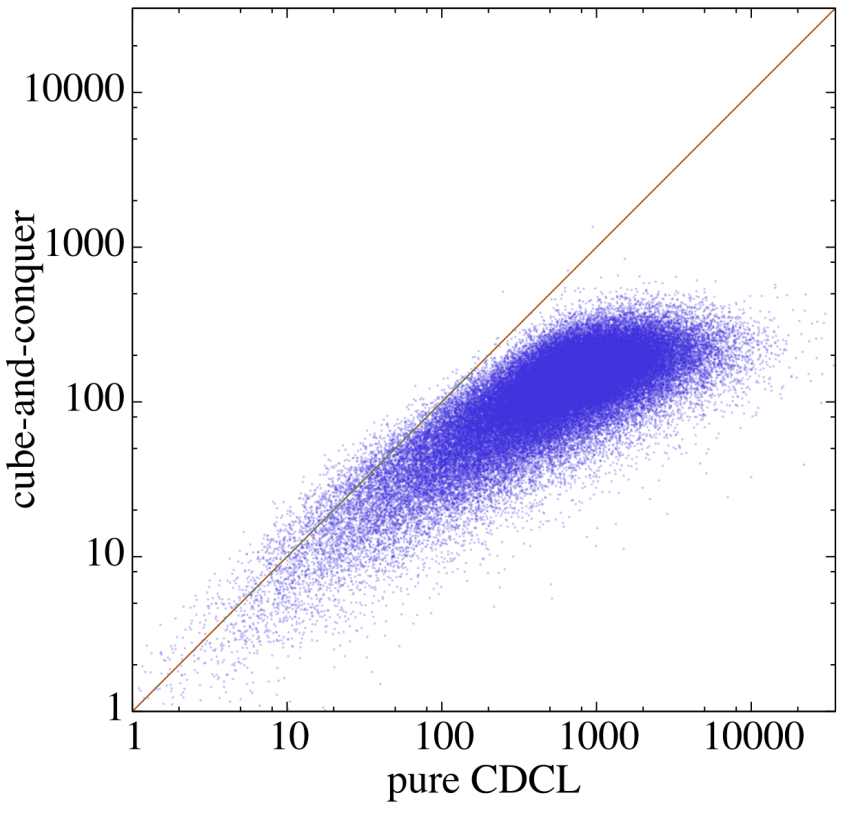
\includegraphics[width=0.5\textwidth]{images/plot1.png} 
		%\caption{runtime of C\&C and CDCL}
	\end{figure}
\end{frame}

\section{Validation}
\begin{frame}{Validation of the program}
	%TODO: add the validation steps
\end{frame}





\end{document}
